\section{Příklad 4}
% Jako parametr zadejte skupinu (A-H)
\ctvrtyZadani{G}

\begin{center}
    \textbf{Krok 1} - Určíme $\omega$, $Z_{L1}$, $Z_{L2}$, $Z_{C1}$, $Z_{C2}$
\end{center}

\begin{gather*}
\omega = 2 \pi f = 2 \pi \times 60 \\
\omega = 120 \pi \\
Z_L = j \omega L \\
Z_C = \frac {1} {j \omega C} \\
Z_{L1} = 52,7787j \Omega \hspace{1cm}
Z_{L2} = 22,6194j \Omega \\
 	Z_{C1} = -16,5786j \Omega \hspace{1cm}
Z_{C2} = -33,1572j \Omega \\
\end{gather*}

\begin{center}
    	\textbf{Krok 2} - Zostaviť rovnice pre smyčkové prúdy $I_A$, $I_B$ a $I_C$
	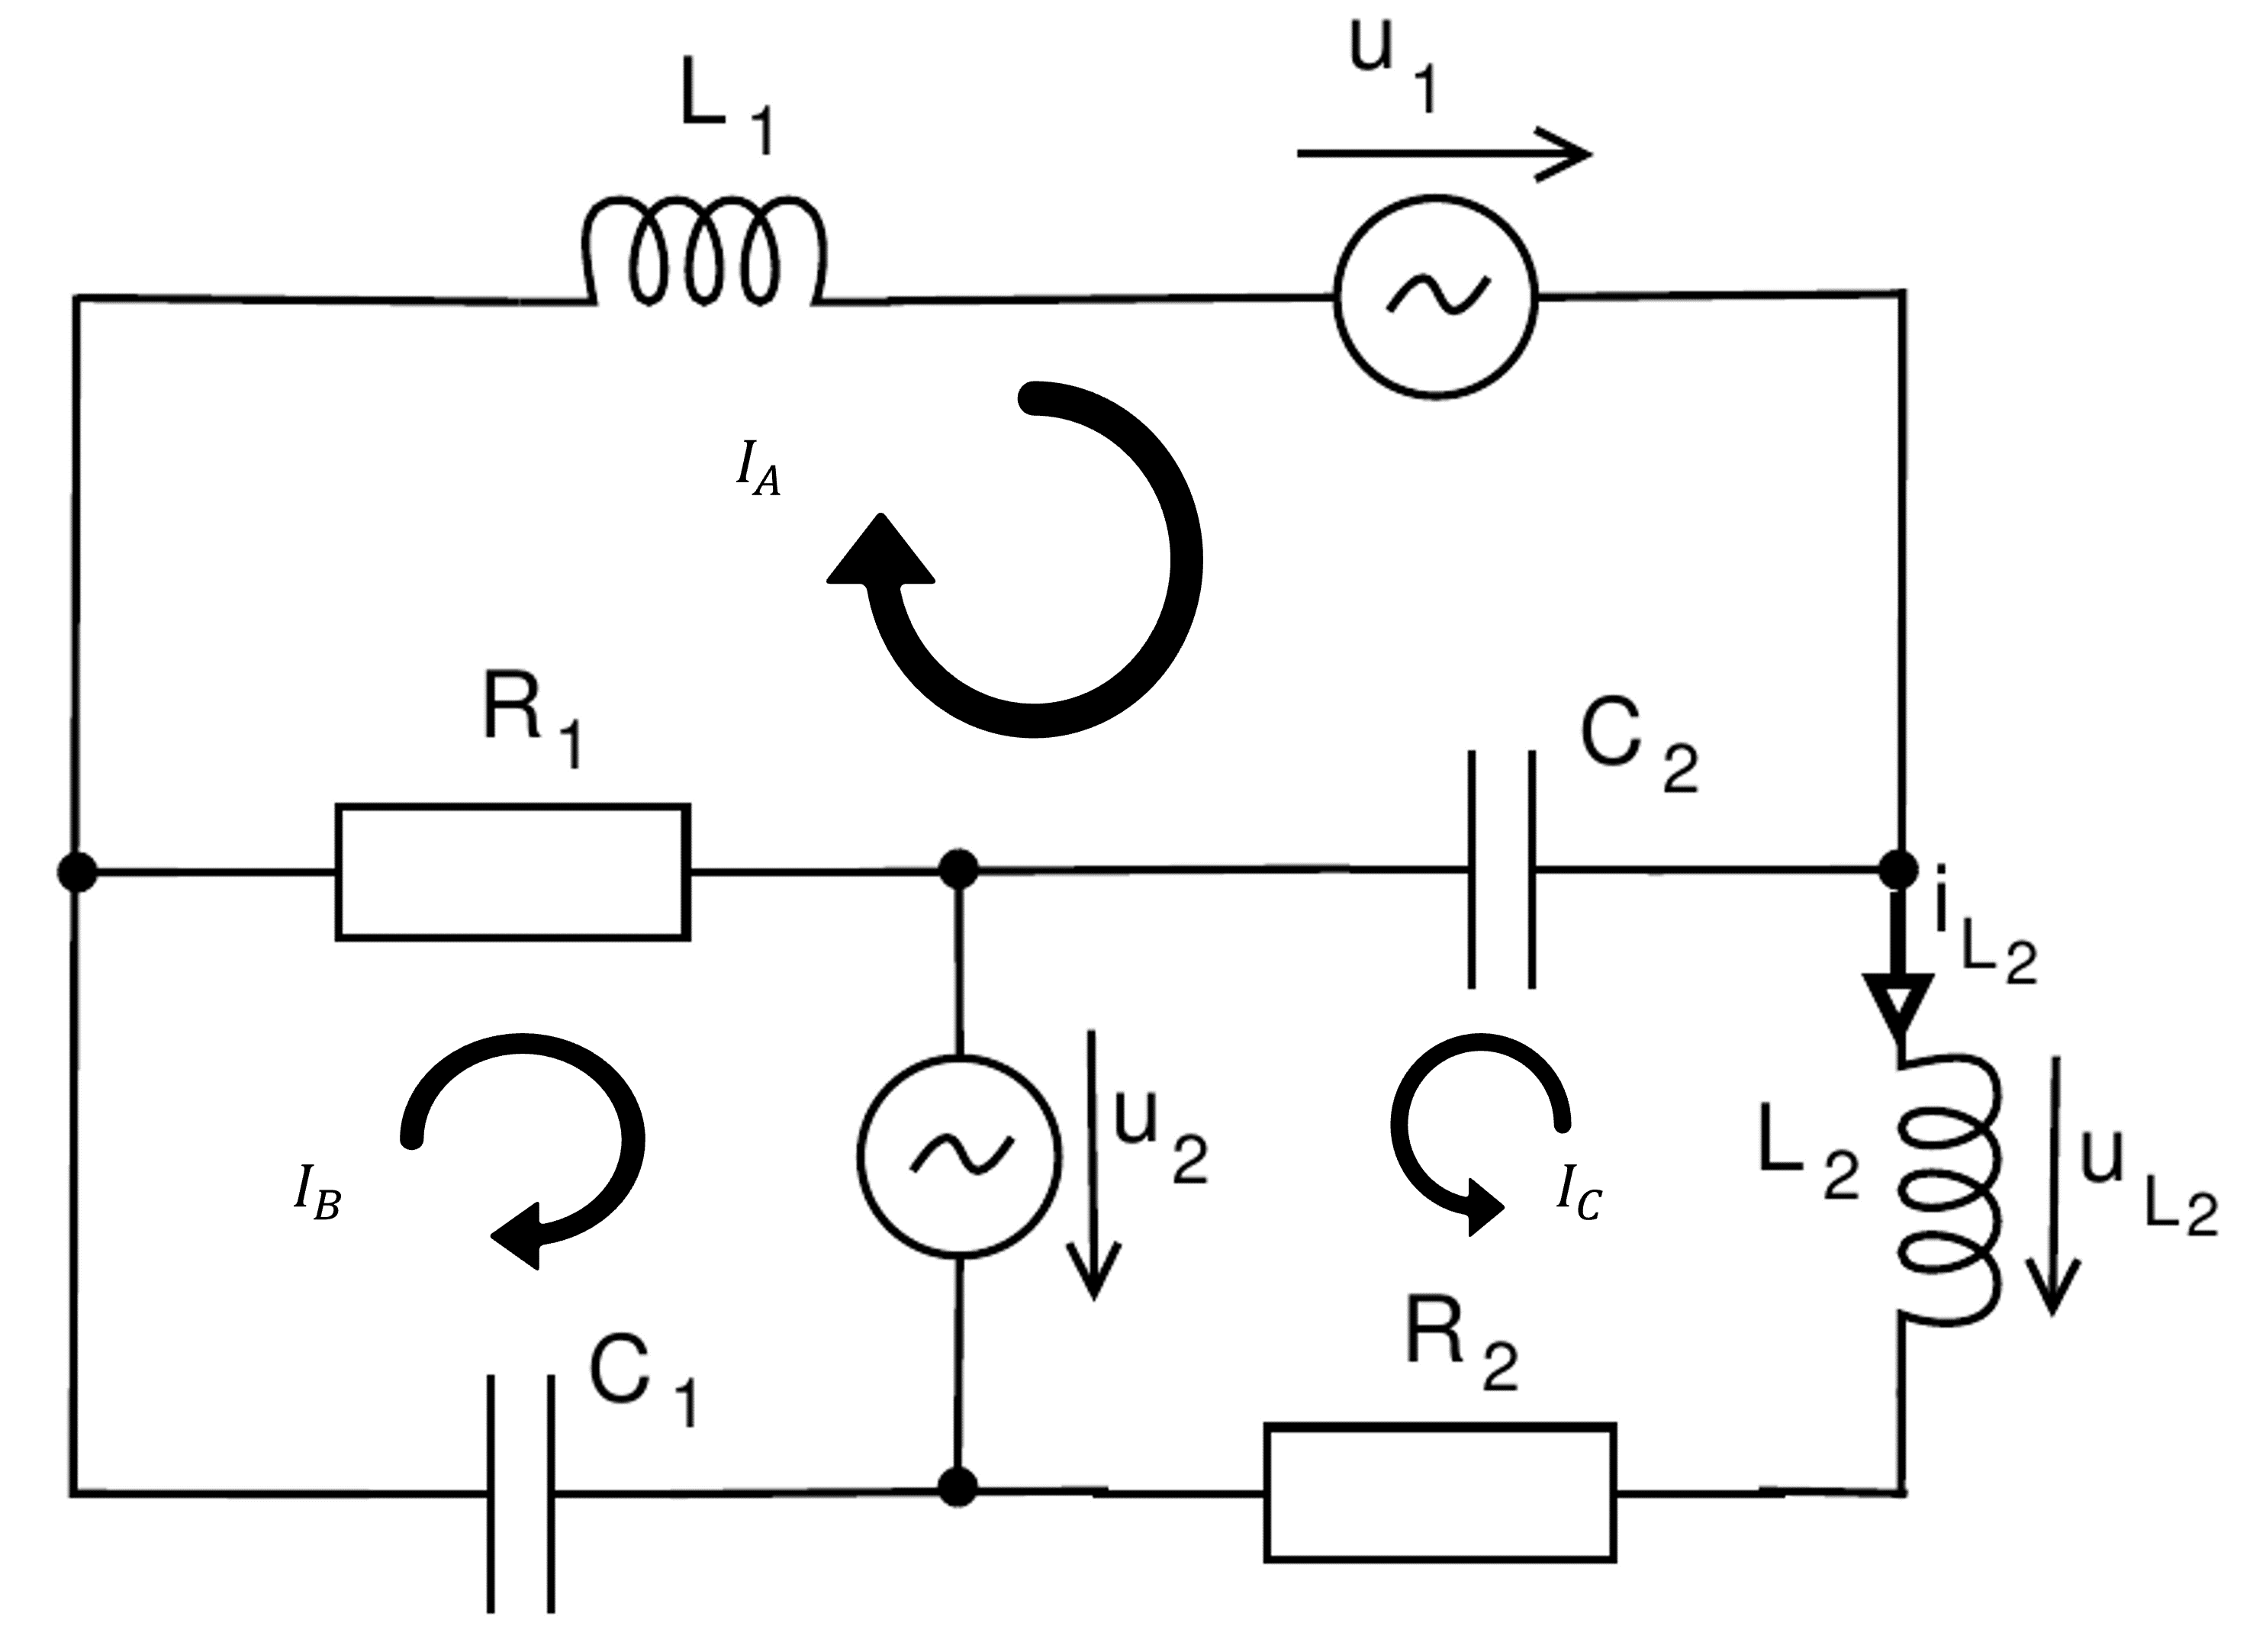
\includegraphics[scale=0.4,keepaspectratio]{fig/pr_4_1.png} \
\end{center}

\begin{gather*}
I_A: I_A(L_1+C_2+R_1) + I_B(-R_1)+I_C(C_2) = -U_1 \\
I_B: I_A(-R_1) + I_B(R_1+C_1) + I_C(0) = -U_2 \\
I_C = I_A(C_2) + I_B(0) + I_C(C_2 + R_2 + L2) = -U_2 \\
\end{gather*}

\begin{center}
    \textbf{Krok 3} - Z rovníc postavíme matice a pomocou Cramerového pravidla a determinantov matíc vypočítame neznámu  $I_C$, ktorú budeme potrebovať na ďalší výpočet
\end{center}

\begin{gather*}
	\begin{pmatrix}
		19,6215j+13 & -13 & -33,1572j \\
		-13 & 13-16,5786j  & 0 \\
		-33,1572j & 0 & -10,5378j+12\\
	\end{pmatrix}
	\times
	\begin{pmatrix}
		I_A \\
		I_B \\
		I_C \\
	\end{pmatrix}
	=
	\begin{pmatrix}
		-5 \\
		-5 \\
		-5 \\
	\end{pmatrix} \\
	\\
	M = 18612,6139-21179.7337j \\
	M_C = -4374,9847-4508,2245j \\
	I_C = 0,0176-0,222098j A \\
\end{gather*}

\begin{center}
    \textbf{Krok 4} - Pomcou vypočítaného $I_C$ vypočítame napätie na cievke $L_2$
\end{center}

\begin{gather*}
U_{L_2} = I_C \times Z_{L_2} \\
U_{L_2} =  0,0176-0,222098j \times   22,6194j = 5,0396 + 0,3998j A \\
U_{L_2} = \sqrt{5,02374^2 + 0,3998^2} = \textbf{5,0396 V} \\
\end{gather*}

\begin{center}
    \textbf{Krok 5} - Vypočítame fázový posun $\varphi$
\end{center}

\begin{gather*}
\varphi C_1 = \arctan{\frac{Im(U_{L_2})}{Re(U_{L_{2}})}} =\arctan{\frac{0,3998}{5,0396}} = 0,0791 rad \\ 
\end{gather*}


